There exist many different graph properties that can be applied depending on the specific graph type. Hence, we will focus on properties that can be applied to connected graphs to provide a collection of values targeted for the same layout structure and giving a wider selection of these such properties. Our aim is to apply these properties onto linguistic graphs (also known as word graphs) to enable the analysis of languages. To accomplish this, each property must be able to calculate their values in a connected graph that can be directed. So, a detailed study of each property will be given and the graphs that they can be applied to. 

\section{Trophic Levels and Coherence}
We begin with the graph property of \emph{trophic coherence} \cite{johnson2014trophic}. In terms of ecology, this property determines the stability of the graph, i.e., the ability that an ecosystem maintains its structure and functions. For example, a food chain \cite{saigo2015trophic} can be represented in levels, higher levels are labelled as predators and lower levels as the prey. Trophic coherence measures whether this structure has clear partitions and uses \emph{trophic levels} to determine their positions within this food chain. Trophic levels are calculated for individual vertices within the graph. The idea of trophic levels are taken from ecology and can be applied to graphs to generate a height-based format for the vertices of a graph. Thus, for a connected directed graph $G =(V,E)$, we have $V$ which is the set of all vertices in $G$ and $E$ which is the set of all the edges within $G$. The graph can be represented with an adjacency matrix $A$ where $a_{ij}$ denotes the elements within the matrix. The standard trophic level definition on vertices uses the in degree and the out degree of the vertex $v_i$ given by Equation \ref{eq:inoutt}.

\begin{equation} \label{eq:inoutt}
k_i^{\text{in}} = \sum_ja_{ij} , \qquad \qquad k_i^{\text{out}} = \sum_ja_{ji} 
\end{equation}

The standard trophic level formula for vertices $v_i \in V$ is defined as:

\begin{equation}
t_i = 1 + \frac{1}{k_i^{\text{in}}}\sum_ja_{ij}t_j
\end{equation}

By ecological convention, $t_i = 1$ if the vertex $v_i$ is \emph{basal}. A vertex is known to be basal if it has no edges directed to it, i.e., $k_i^{\text{in}} = 0$. The trophic level equation can also simply be written in matrix form by Equation \ref{eq:mtl} with $\bold{z}$ defined as $z_i = \text{max}(k_i^{\text{in}},1)$ and $\Delta = \text{diag}(\bold{z}) - A$.

\begin{equation} \label{eq:mtl}
\Delta\bold{t} = \bold{z} 
\end{equation}

All vertices will receive a trophic level if and only if the Laplacian matrix $\Delta$ is invertible as the row sum of elements in $\Delta$ equals 0 for non-basal vertices. If there are no basal vertices in the graph then $\Delta$ will be equal to the zero matrix and thus be singular, i.e., no inverse. This is discussed by Johnson \cite{johnson2020digraphs} in the investigation of stability and such dynamical features within graphs. So, for standard trophic levels equation to be applicable for the entire graph, there must exist at least one basal vertex meaning that this is a limitation to the definition of trophic levels. In the case of linguistic analysis, a basal vertex exists because sentences will always have a word that is the start, i.e., a vertex without any in edges. However, in a larger dataset, the starts of sentences may be used in other areas meaning that they are no longer basal. Consequently, we study the improved equation for trophic levels and the possibility of weight inclusion. 

\subsection{Inclusion of weights and equation improvement}
In a weighted graph $G = (V, E)$, edges carry a weight between a vertex $v_i$ to a vertex $v_j$ where $i , j = 1 , 2, \dots , \lvert V \rvert$. Weighted matrix $W$ are used as a representation of the entire graph along with incorporating the direction of each edge and self-loops if they exist. The elements of the weighted matrix are $w_{ij}$. If the graph is not weighted then the edge is valued as 1 if the edge exists and 0 otherwise, i.e., the adjacency matrix of G. The total weight (also known as the \emph{strength}) for each vertex is defined by the weights into a vertex $v_i$ and the weights out of vertex $v_i$, which is shown by $s_{v_i}$ in Equation \ref{eq:strength}. This is essentially the same as the in and out degrees of Equation \ref{eq:inoutt} mentioned previously but instead of 1s and 0s, the weighted values are considered. The imbalance of the vertex $v_i$ is defined by the weights in of a vertex minus the weights out of the vertex shown by $i_{v_i}$ in Equation \ref{eq:imb}.

\begin{align}
s_{v_i} &= \sum(w_{v_iv_j}) + \sum(w_{v_jv_i}) \label{eq:strength} \\
i_{v_i} &= \sum(w_{v_iv_j}) - \sum(w_{v_jv_i}) \label{eq:imb}
\end{align}

Vectors $\bold{s}$ and $\bold{i}$ hold all the values of the strength and imbalance for all vertices respectively. We let $\bold{h}$ be a vector, then the graph Laplacian operator in matrix form is defined by Equation \ref{eq:delt}.  

\begin{equation} \label{eq:delt}
\Delta = \text{diag}(u) - W - W^T
\end{equation}

Therefore, to get the trophic levels for each vertex with consideration for the additional weights, we solve the system of equations for vector $\bold{h}$ as shown by Equation \ref{eq:h}.

\begin{equation} \label{eq:h}
\Delta \bold{h} = \bold{v} 
\end{equation}

The values within this vector $h$ correspond to the trophic levels for the relative vertices. The values are used to illustrate the various trophic levels within a graph to give a hierarchical format visualisation. Trophic levels are not unique solutions because an arbitrary constant can be added to each component of the graph if there are multiple components to generate new levels that would be correct. The benefit to this is that Equation \ref{eq:h} can use an arbitrary constant $c$ for a vertex in $\bold{h}$ to influence the value of other vertices in a component. If there are multiple components to the graph, then a vertex in each component is needed. A unique solution can be found this way in which the trophic level values can be shifted so that a better graphical display can be generated. For example, having the lowest trophic level to be 0. 

Trophic levels can also be used to equate the overall \emph{trophic incoherence} of the graph rather than just looking at the graph on a vertex level. By using the trophic levels from $\bold{h}$, the equation for the trophic incoherence is defined by MacKay, Johnson, Sansom \cite{johnson2020digraphs} to be:

\begin{equation}
F_0=\frac{\sum_{v_iv_j}w_{v_iv_j}(h_{v_j}-h_{v_i}-1)^2}{\sum_{v_iv_j}w_{v_iv_j}}
\end{equation}

The possible shifting of the trophic levels does not affect the trophic incoherence meaning that the equation is independent. The incoherence is strictly ranged from 0 to 1. If $F_0 = 0$  then the graph is \emph{maximally coherent}, as it would mean that all levels in the graph have a precise equal spacing which means that the graph is perfectly separated into levels. Whereas if $F_0 = 1$ then the graph is \emph{maximally incoherent} and levels are harder to decipher. As $F_0$ measures the incoherence, by taking $1 - F_0$, this would instead measure the coherence of the graph as they are each other's converses. 
\newline

In conclusion, trophic levels can be applied to weighted directed graph and any subcategories to achieve a hierarchical view of the graph. This eases the visualisation of many datasets and is used to decipher valuable information that may be of use. Through the combination of other graph properties which are described in this chapter, various combinations of these properties will yield different visualisations. This will prove beneficial in finding key vertices and correlations when analysing various languages. Through using trophic levels in languages, the graph can be formatted to demonstrate the sentence structure visually. Additionally, as shifting their trophic values does not affect the overall coherence, values can be modified so 0 indicates the start of the sentence and larger values indicate positions further up the sentence.

\section{Clustering Coefficient}
The \emph{clustering} of a graph, also known as \emph{transitivity} \cite{schank2005approximating}, is a property of a graph that measured the density of triangles within the graph. Triangles are where 3 vertices are connected. Clustering is used to quantify the graph's connectivity strength as it determines the fraction of triangles over the possible triangles that could be formed within the graph. Another perspective is that the coefficient quantifies the probability of a vertex $a$ having an edge to vertex $c$ if $ab$, $bc \in E(G)$. Thus, the \emph{clustering coefficient} determines how complete the graph is with a value of 1 meaning it is complete and 0 if not. There are two popular introductions of clustering coefficient, the \emph{local clustering}, and the \emph{global clustering}. The global clustering coefficient essentially measures the completeness of the graph by measuring the number of existing triangles divided by the number of possible triangles. The local clustering coefficient measures the clustering coefficient for each vertex rather than the whole graph. The measurement is taken by the number of triangles that have a connection to this vertex over the number of triples centred on this vertex. In other words, the local value demonstrates how close the neighbours of this vertex are to being a complete graph (a \emph{clique}).

\subsection{Clustering for simple graphs}
For simple connected graphs that are unweighted and undirected, we determine the coefficients of the clustering. The global clustering coefficient is defined by equation \ref{eq:sgcc} where $\sum{T}$ denotes the number of triangles (closed triplets) and $\sum{\tau}$ denotes the number of connected triplets in the graph.
\begin{equation} \label{eq:sgcc}
C = \frac{3\text{(Number of all triangles)}}{\text{Number of all connected triples}} = \frac{\sum{T}}{\sum{\tau}}
\end{equation}
An alternative equation which was demonstrated by M.E.J. Newman \cite{Newman_2003} through the studies of complex networks in terms of social networks. This is where the clustering coefficient determines the likelihood that a friend of your friend is also your friend. So, the alternative equation is written in the form of equation \ref{eq:sgccp} where $\sum{P_2}$ denotes the number of paths with length two within the graph.
\begin{equation} \label{eq:sgccp}
C = \frac{6\text{(Number of total triangles)}}{\text{Number of paths with length 2}} = \frac{\sum{T}}{\sum{P_2}}
\end{equation}

By considering the vertices of the graph, the local clustering coefficient can be defined to give such a coefficient to each vertex $v\in V(G)$ and is achieved by the equation \ref{eq:slcc} where $i$ is the index of the vertex. This definition is from paper \cite{Newman_2003} and proposed by Watts and Strogats \cite{Watts1998} where they analysed small world networks in relation to various real-world systems using clustering coefficients and random graphs to formulate certain similarities. Note that if the degree of a vertex is 1 then the coefficient can be determined as 0, otherwise the equation will lead to $0/0$.
\begin{equation} \label{eq:slcc}
C_i = \frac{\text{Number of triangles connected to vertex $i$}}{\text{Number of triples centred on vertex $i$}}
\end{equation}

Another representation of the global clustering coefficient is to take the averages of all the local coefficients \cite{https://doi.org/10.48550/arxiv.1410.1997}. When the vertices have a degree of 0 or 1 then $C_i = 0$ so global clustering coefficient can also be defined by equation \ref{eq:sglcc}.
\begin{equation} \label{eq:sglcc}
C = \frac{1}{n}\sum_i{C_i}
\end{equation}
Later the clustering coefficients will be used as assistance to model graphs generated from a language dataset. However, to provide more accurate coefficients, variations of the clustering formulas will be defined based on the inclusion of weights and/or directions. In terms of our goal of linguistic analysis, directions are of key importance since the word graphs will be directed. Therefore, the definitions of clustering coefficients must be developed further, starting with a overview of the inclusion of weighted edges.

\subsection{Clustering for weighted graphs}
Now by considering graphs as before but weighted instead, the equations undergo changes. For the instance of weighted graphs, there are multiple different definitions of clustering coefficients, each with slight variation in coefficients. This section will summarise a couple of the different definitions for weighted graphs and further detail can be analysed from Tanguy and Anna Levina on weighted directed clustering \cite{PhysRevResearch.3.043124}. In this paper, four different definitions are reviewed which are the Barrat definition, Onnela's definition, Zhang \& Horvath and their own continuous definition for weighted graphs. Zhang \& Horvath \cite{ZhangHorvath+2005} have used their definition of weighted clustering coefficients to analyse gene co-expression networks to review their functionality. Additionally, by soft or hard thresholding, it enables them to determine relationships between the clustering coefficient and gene networks within biology.

Alternatively, a simple idea to associate the clustering coefficient with regards to the edge weights is to define a value $w$ that represents the value of the triplet. $w$ can be the summation of the triplet, the mean of the triplet or another suitable method depending on the purpose. We take $w$ to be the summation of edges of the triplets. Then Equation \ref{eq:wcc} calculates the weighted clustering coefficient \cite{opsahl2009clustering} where $T$ denotes the triangles in the graph and $\tau$, the triples.
\begin{equation} \label{eq:wcc}
C = \frac{\text{Total of closed }w}{\text{Total of }w} = \frac{\sum_T{w}}{\sum_\tau{w}}
\end{equation}

\subsection{Clustering for directed graphs}

We see that weights can be added trivially through Equation \ref{eq:wcc}. So now considering the addition of directions as well as the possibility of weighted edges. Directions cause further complexities in the coefficients of clustering due to the various number of different \emph{motifs}. Motifs are various patterns in graphs that are reoccurring and can be used here to describe the nature of the triangles. For instance, there are 16 possible motifs for directed graphs of 3 vertices shown in Figure \ref{fig:3nodes}. However, if we consider only connected triangles, they can be organised into 4 types of motif groups known as \emph{Cycles}, \emph{Middleman}, \emph{Fan-in}, and \emph{Fan-out}. Demonstrated by Figure \ref{fig:change} which are used in the study of higher order motifs and synaptic integration by Bojanek, Zhu and Maclean \cite{synaptic}. An interesting result used in this paper is the isomorphisms between the middleman, fan-in, and fan-out motifs.

\begin{figure}[!htb]
	\centering
	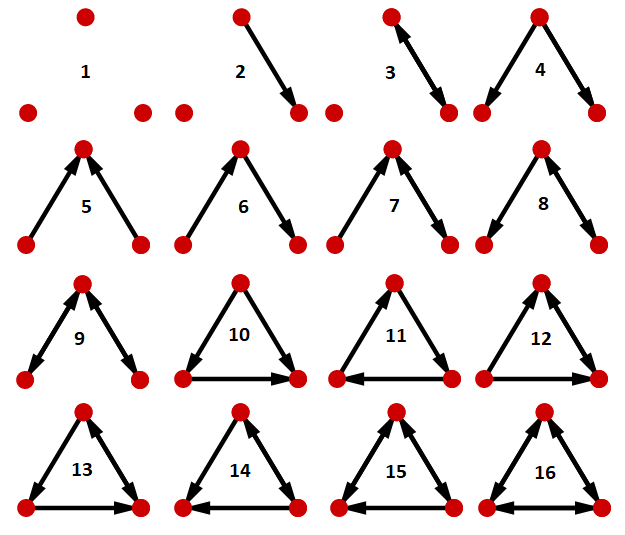
\includegraphics[scale=0.6]{3nodes}
	\caption{All 16 motifs of possible connections between 3 nodes and their directions shown on the edges. Ranges from 0 directed edges to the maximum of 6 directed edges.}
	\label{fig:3nodes}
\end{figure}

\begin{figure}[!htb]
	\centering
	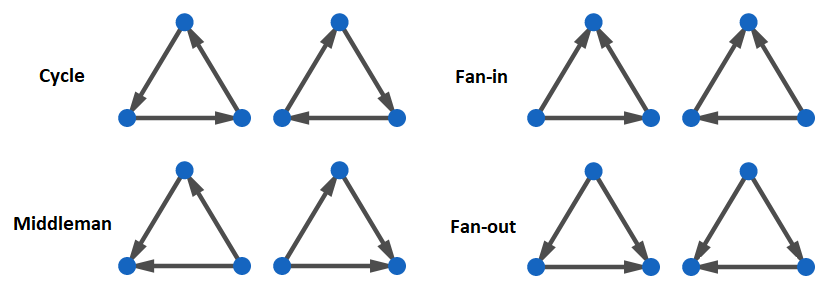
\includegraphics[scale=0.6]{change}
	\caption{The 4 named categories of motifs in which all directed connected triangles fall under. Each pair of motifs is listed as the corresponding types which are cycles, middleman, fan-in, and fan-out.}
	\label{fig:change}
\end{figure}

Consideration of the directional edges yields better accuracy in the coefficient values. One of the versions mentioned in the paper \cite{PhysRevResearch.3.043124} was Fagio's where he introduces the clustering coefficient to binary directed networks which are equivalent to simple directed connected graphs. Firstly, the equation for the directed version without the consideration of weights is defined by the ratio of all directed triangles centred on a vertex $i \in V(G)$ over the number of all possible triangles that could be formed with vertex $i$. Which are called $t_{i}$ and $T_{i}$ respectively. Before the directed equation for clustering, prior properties of the graph are necessary so that the equation can be easily formulated. Thus, consider a graph $G = (V, E)$ with its matrix representation as the adjacency matrix $A$ along with $V_1$ as the column vector, dimension $n$ of the graph, of only 1s. $A_i$ is the $i$-th row of the adjacency matrix. The in-degrees and out-degrees of a graph are the total number of edges going in or out of a vertex $i\in V(G)$ respectively, the total degree is the sum of the in and out degrees shown by Equations $\ref{eq:idod}$.

\begin{align} \label{eq:idod}
\text{in}(d_i) &= \sum_{i\neq j}a_{ji} = (A^T)_i V_1 \\
\text{out}(d_i) &= \sum_{i\neq j}a_{ij} = (A^T)_i V_1 \nonumber \\
\text{tot}(d_i) &= \text{in}(d_i) + \text{out}(d_i) = \sum_{i\neq j}a_{ji} + \sum_{i\neq j}a_{ij} = (A^T + A)_i V_1 \nonumber
\end{align}

When the edge is directed both ways, this degree is the summation of the products of all the edges of vertex $v$ that are bidirectional. Formally can be shown as equation \ref{eq:bd} with $A_{ii}$ as the $i$-th element of the diagonal for the matrix product of $A$.

\begin{equation} \label{eq:bd}
\text{bi}(d_i) = \sum_{i\neq j}a_{ij}a_{ji} = (A^2)_{ii} 
\end{equation}
 
Equation \ref{eq:dcc} is demonstrated by Fagio \cite{Fagiolo_2007} that measures the local clustering coefficient for each vertex with directed edges. Amended based on the consideration of the 8 triangles that this vertex could form shown previously in Figure \ref{fig:change}. 

So, this equation can be demonstrated with vertex $i$ and pairs of neighbours $j$ and $k$. Essentially showing that Equation \ref{eq:dcc} calculates the triangles formed by $v$ over all possible triangles with the deduction of $2\text{bi}(d_i)$. The deduction is necessary. Otherwise, if vertex $i$ and vertex $j$ have edges directed to each other, this causes a count of two additional triangles due to the nature of bidirectional edges.

\begin{align} \label{eq:dcc}
C_i &= \frac{\frac{1}{2}\sum_j \sum_k (a_{ij} + a_{ji})(a_{ik} + a_{ki})(a_{jk} + a_{kj})}{\text{tot}(d_i)(\text{tot}(d_i) - 1) - 2\text{bi}(d_i)} \\
&= \frac{(A + A^T)^3_{ii}}{2(\text{tot}(d_i)(\text{tot}(d_i) - 1) - 2\text{bi}(d_i))} = \frac{t_i}{T_i} \nonumber
\end{align}

Weights of the edges can be implemented into Fagio's equation of local clustering coefficients by simply using a weighted adjacency matrix $W$ instead of the adjacency matrix $A$ for graph $G$. Mentioned before, the weights of the triangles can be considered differently. However, in Fagio's generalisation of the local clustering coefficient equation, the mean weights of the triangles are utilised. This is shown by taking a cube root of all elements of the weighted matrix $W$ which can be denoted as $W^{[1/3]}$. Therefore by subbing $W^{[\frac{1}{3}]}$ in the place of $A$ in Equation \ref{eq:dcc}, the weighted directed version can be achieved, formally shown as Equation \ref{eq:wdcc}.

\begin{equation} \label{eq:wdcc}
C_i = \frac{(W^{[\frac{1}{3}]} + (W^{[\frac{1}{3}]})^T)^3_{ii}}{2(\text{tot}(d_i)(\text{tot}(d_i) - 1) - 2\text{bi}(d_i))} = \frac{t_i}{T_i}
\end{equation}

However, with this generalisation of the formula, it considers any triangle formed by a vertex $i$ as equal values. This means that the directions in the triangles are meaningless when utilising this equation. For directed graphs, their directions are what gives the graph its flow of information and different directions will lead to different interpretations of the graph. Consequently Equation \ref{eq:wdcc} must be improved to properly include the directions of edges and to consider each motif separately. In Fagio's case, treat them by considering the 4 types of categories the motifs can fall under mentioned before in Figure \ref{fig:change}. 

The 4 motifs were cycles, middleman, fan-in, and fan-out. By measuring each specific category, we can get more accurate coefficients for the relative pattern. The definition of the number of all possible triangles was defined in equations \ref{eq:dcc} and \ref{eq:wdcc} as $T_i$. Similarly with the directed triangles that are formed by a vertex $i$ as $t_i$. These can be both decomposed into the 4 types of motifs which can then be used to create the local clustering coefficient for each specific motif. Note that the sum of the local clustering coefficient for each specific motif will equal the local clustering coefficients for all triangles. The equations are decomposed as follows:

\begin{align}
T_i &= \text{tot}(d_i)(\text{tot}(d_i) - 1) - 2\text{bi}(d_i) \\
&= \text{in}(d_i)\text{out}(d_i) - \text{bi}(d_i) + \text{in}(d_i)\text{out}(d_i) - \text{bi}(d_i) \nonumber \\
&+ \text{in}(d_i)(\text{in}(d_i) - 1) + \text{out}(d_i)(\text{out}(d_i) - 1) \nonumber \\ 
&= \text{cyc}(T_1) + \text{mid}(T_2) + \text{fan-in}(T_3) + \text{fan-out}(T_4) \nonumber
\end{align}

\begin{align}
t_i &= (W^{[\frac{1}{3}]} + W^T)_{ii} \\
&= ({W^{[\frac{1}{3}]})}^3_{ii} + (W^{[\frac{1}{3}]}{W^{[\frac{1}{3}]}}^TW^{[\frac{1}{3}]})_{ii} + ({W^{[\frac{1}{3}]}}^T{W^{[\frac{1}{3}]}}^2)_{ii} + ({W^{[\frac{1}{3}]}}^2{W^{[\frac{1}{3}]}}^T)_{ii} \nonumber \\ 
&= \text{cyc}(t_1) + \text{mid}(t_2) + \text{fan-in}(t_3) + \text{fan-out}(t_4) \nonumber
\end{align}
 
Both equations can be split according to their different motifs through logical and algebraic reasoning. For $T_i$, the maximum number of directed triangles for cycles, middleman, fan-ins, and fan-outs that can be formed equates to the total number of triangles for a vertex $i$. For example, when calculating cycles, the maximum number of directed cycles that can be formed with vertex $i$ is the number of edges into the vertex multiplied by the number of edges out, hence giving $\text{in}(d_i)\text{out}(d_i)$ in the equation. Although, if a neighbour of vertex $i$ has an edge to and from another vertex then this would account to an additional triangle counted. So, the subtraction of the bidirectional edges,  $\text{bi}(d_i)$, remains necessary. Notice that middleman and cycles are only differentiated by the direction of the pairs of neighbours connected to vertex $i$ which forms the triangle. This is the reason why $\text{cyc}(T_1) = \text{mid}(T_2)$. Then for the calculations of fan-in motif, it is the multiplication of the in degrees of $i$ and in degrees of $i - 1$ (as an edge is already considered) which gives the maximum fan-in motif styled triangles. Similarly for the fan-out motif.

Then for the actual triangles formed, they can be broken down by algebra. Equation \ref{eq:cyca} breaks down the calculations for actual cycles based on the motif of 3 vertices. The others follow a similar process. Hence by algebraic manipulation, $t_i$ can be separated into the 4 motifs shown before.

\begin{align} \label{eq:cyca}
\text{cyc}(t_i) &= \frac{1}{2}\sum_j\sum_h{w_{ij}w_{jh}w_{hi} + w_{ih}w_{hj}w_{ji}} \\
&= \frac{1}{2}((W^{[\frac{1}{3}]})_{(i)}W^{[\frac{1}{3}]}(W^{[\frac{1}{3}]})^{(i)} + (W^{[\frac{1}{3}]})_{(i)}^T(W^{[\frac{1}{3}]})^T(W^{[\frac{1}{3}]})(W^{[\frac{1}{3}]})^{(i)}  \nonumber \\
&= (W^{[\frac{1}{3}]})_{(i)}W^{[\frac{1}{3}]}(W^{[\frac{1}{3}]})^{(i)} = ({W^{[\frac{1}{3}]})}^3_{ii} \nonumber
\end{align}

Finally, the local clustering coefficient can be calculated according to the specific motifs of cycles, middleman, fan-in, and fan out. Which can be formally defined as:

\begin{equation} \label{eq:wdmcc}
x(C_i) = \frac{x(t_i)}{x(T_i)}
\end{equation}

where $x$ = \{cyc, mid, fan-in, fan-out\} .\\

By demonstrating one specific formulation of the local clustering coefficient applied to weighted directed graphs, we notice that depending on variations of properties in relation to the triangles, different values may occur for the same graph. Such properties include the various different motifs of the triangles and the consideration of the edge weights. This is reason why there exists multiple different versions of clustering calculations as each has their benefit depending on what the graph represents. The different versions of clustering formula are thoroughly examined in the paper \cite{PhysRevResearch.3.043124}. Additionally, all versions can also be analysed against each other to determine which has the best performance depending on the ideal requirements of the task \cite{CLEMENTE201826}.

For the goal of linguistic analysis, we will initially take the calculations of the local clustering coefficients for directed graphs. So that we can determine if vertices form a relationship with specific areas of the text or with individual words. Using local clustering coefficient will help determine which words are important in its local cluster. Additionally local clustering can help visualise the various clusters in a word graph and identifies the graph's completeness. Note that the possibility of patterns may also occur when analysing the word graph since the clustering coefficients utilises triangles in a graph. 

\section{Centrality}
Positioning within a graph is vital in displaying information in a simple manner. We want the positions to be useful for extracting important information. Key benefit of useful positioning is that the positions may be used to identify key areas within a graph or network such as the links between companies and which one has the most influence. This can also be applied to brain networks, the spreading patterns of disease and is useful to characterise specific areas to give a new interpretation of the graph. To assist in accomplishing a better positional system for graphs, we look at centrality values. Centrality values focus on the vertex location amongst its neighbours or connections within the whole graph. Assigning numerical values to them depending on their importance or usefulness. One of the major centrality values is the betweenness centrality of vertices in a graph which will be described in further detail in the next section.

\subsection{Betweenness centrality}
\emph{Betweenness centrality} measures the centrality of a graph by using the shortest paths for pairs of vertices. It identifies vertices who are most influential within the graph, i.e., vertices that are required in the paths of other vertices. The introduction of this idea was through the view of a communications network. Where a vertex (or point) of the communications network is deemed to be central if it lies on the shortest path between another pair of vertices. Alex Bavelas \cite{bavelas1948mathematical} formularised this idea of centrality where he suggests that a person in a group is in the central position if that person lies on the shortest path between other connecting pairs. With the implication that this person then holds the power or responsibility for the others. Due to the fact that when exchanging information, the others must go through that person. A simplistic way of viewing the betweenness value for a vertex is that the larger the value, the greater number of shortest path connections it has to other vertices. In other words, if the value is large for a vertex, then the travel time from this vertex to other vertices is much shorter. 

The betweenness centrality will be discussed based on Freeman's interpretation of betweenness centrality measure \cite{freeman1977set}. For a simple unconnected and undirected graph $G = (V, E)$, consider all the unordered pairs of vertices $v_i, v_j \in V$ with $i \ne j$. This pair must either be disconnected or have at least one path connecting them with its path length based on the number of edges contained within. The path or paths connecting $v_i$ to $v_j$ with the shortest length is known to be \emph{geodesic}. If the path is larger than one edge (the vertices were adjacent) then vertices in this geodesic are central. Depending on whether the vertex is the only central vertex between the pair of vertices determines if it has complete or partial control of their link. The intuition of control in betweenness was expressed by Shimbel \cite{shimbel1953structural} where work sites are considered as vertices. Meaning that the vertices with control will be the connecting sites between other sites. Which in terms means that the connecting sites hold responsibility to the other sites and must relay information and resources to them. Figure \ref{fig:geodesics} expresses the idea of central vertices and the geodesics between them. For the path between vertices $v_1$ and $v_3$, there are 2 shortest paths of length 3 which means they have 2 geodesics. Suggesting that there could be up to 2 vertices which share the power of information transfer between vertices 1 and 3. Another example is that vertices $v_3$ and $v_6$ only have one geodesic through $v_4$ and $v_0$ so either $v_4$ or $v_0$ can have complete control of power.

\begin{figure}[!htb]
	\centering
	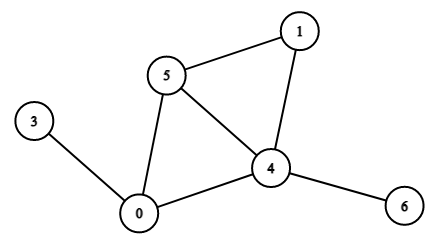
\includegraphics[width=.7\linewidth]{geod.png}
	\caption{A simple graph of 6 vertices and 7 edges. Vertices $v_1$ and $v_3$ have two geodesics meaning that the central vertices are $v_4$ and $v_5$ who share partial control but $v_0$ has full control and is most central between $v_1$ and $v_3$. Note that $v_3$ and $v_6$ cannot be central as they only have one edge each and they only have one geodesic because if $v_5$ or $v_1$ is included then it is no longer the shortest path between $v_3$ and $v_6$.}
	\label{fig:geodesics}
\end{figure}

If there is more than one geodesic, then they are considered to have equal probability in deciding which one to be used. This is simply given by $1/g_{ij}$ where $g_{ij}$ is the number of geodesics between vertices $v_i$ and $v_j$. The formalisation of partial betweenness $b_{ij}(v_k)$ is defined using the idea of geodesics, so for a vertex $v_k$ in $G$ and a vertex pair $v_i$ and $v_j$, the partial betweenness for $v_k$ can be calculated based on the vertex pair and is given by Equation \ref{eq:gb}.

\begin{equation} \label{eq:gb}
b_{ij}(v_k) = \frac{1}{g_{ij}}(g_{ij}(v_k)) = \frac{g_{ij}(v_k)}{g_{ij}} (i \ne j \ne k)
\end{equation}

where $g_{ij}(v_k)$ is the number of geodesics connecting vertices $v_i$ and $v_j$ that include $v_k$ in its path. This essentially translates to the probability that the geodesic chosen for $v_i$ and $v_j$ contains $v_k$. Additionally, notice that $b_{ij}(v_k) = 0$ if there does not exist a path between the vertex pair, $v_i$ and $v_j$ using $v_k$.
This equation can be extended to calculate the betweenness centrality of each vertex. So, for a graph of size $n$, the betweenness centrality value for a vertex $v_k \in V$ is be defined by Equation \ref{eq:cdvk}.

\begin{equation}\label{eq:cdvk}
C_B(v_k)= \sum_i^n\sum_j^n b_{ij}(v_k)
\end{equation}
where $i < j$. This defines the betweenness centrality for $v_k$ and its value increases depending on the number of geodesics that $v_k$ is a part of. The maximum value \cite{freeman2002centrality} was proved by Freeman using a star graph with the central vertex as $v_k$ as all vertices are reachable if they go through the central vertex. Furthermore, this means there are $n(n-1)/2$ paths between all the unordered pairs of the star graph $S$. With $n-1$ edges connected to the central vertex $v_k$. Thus, the betweenness centrality for $v_k$ in $S$ is

\begin{equation}
C_B(v_k)= \frac{n(n-1)}{2} - (n-1) = \frac{n^2-3n+2}{2}
\end{equation}

And if any new edge is added that does not increase the branches of the star, then a new geodesic would form without $v_k$ causing the betweenness of $v_k$ to fall. Therefore Equation \ref{eq:bcrmv} expresses the betweenness centrality of any vertex in a graph $G$ by its representation through a ratio with the maximal value as shown using the star graph S.

Directed edges are required in linguistic analysis so we study the use of betweenness centrality and its equations for directed graphs as well.

\begin{equation}\label{eq:bcrmv}
C'_B(v_k)= \frac{2C_B(v_k)}{n^2-3n+2}
\end{equation}

\subsection{Generalisation to directed graphs}
The key idea of betweenness centrality is to evaluate the graph and produce values based on the shortest paths of all the possible pairs of the graph. The higher the betweenness value, the more likely the vertex is on the shortest paths of any two vertices. As this concept investigates the vertices on shortest paths, weighted edges would not benefit this graph evaluation as weights could cause a pair of vertices to be seen as further apart than they are within the graph. Also, for experimentations done later with word graphs, the calculations for betweenness will benefit on edges without weights. As the weights may influence the paths of edges between words when the words have a strict order within a sentence. Nonetheless a brief overview of weight inclusion is given.

In the experimentations of social networks \cite{freeman1979centrality}, the centrality values are used on undirected graphs however an idea to generalise the betweenness to weighted graphs is to take the weights as indication of the distance of the vertices. Meaning that the geodesics of any pair will be defined on the smallest total value of paths between them rather than the shortest path length as shown on Figure \ref{fig:dbc}.

\begin{figure}[!htb]
	\centering
	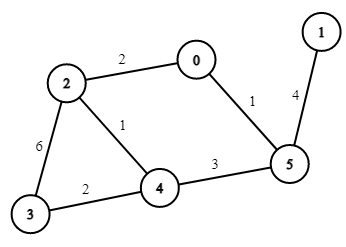
\includegraphics[width=.7\linewidth]{weightedbetween.png}
	\caption{Shows a simple weighted graph. The path between vertex $v_0$ and $v_3$ has 1 geodesic but when considering the weights, this geodesic has a weight of 6. The smallest weighted geodesic is using the path $v_0v_2v_4v_3$ with a weight of 5 instead of the original geodesic. }
	\label{fig:dbc}
\end{figure}

Since weighted edges do not benefit the word graphs when considering centrality, we discuss the generalisation in this section only to directed graphs. If the graph has weights, then they are not implemented to ensure betweenness values will not be influenced and remain congruent throughout experimentation. The geodesic proportions of paths from $v_i$ and $v_j$ was defined earlier in Equation \ref{eq:gb}. Consequently, this equation can be utilised to define pair-dependency of vertices $v_i$ to $v_k$ where the vertex $v_i$ must depend on vertex $v_k$ in order to get to other vertices such as $v_j$ on its geodesics. In other words, $v_k$ acts like a gatekeeper to $v_i$. Therefore, for a graph with $n$ vertices, the pair dependency is defined to be 

\begin{equation}\label{eq:bcrmv}
d^*_{ik} = \sum_{j=1}^{n}b_{ij}(v_k)
\end{equation}

where $i \ne j \ne k$. Matrices can be used to store the pair-dependency values to provide ease of use and a better representation for all values. The results can be arranged into the matrix $D$ defined as $D = (d^*_{ik})$. The elements of the matrix measures how much the vertex $x$ (corresponding to the row number) depends on vertex $y$ (corresponding to the column number) to connect to other vertices in the graph. Additionally, the betweenness centrality can also be calculated based on this matrix $D$ through the summation of the columns in which the sum will give the betweenness centrality for the column number that represents the vertex. Otherwise shown as

\begin{equation}
\sum_{i=1}^nd^*_{ik} = 2C_B(v_k)
\end{equation}

Which means that the betweenness centrality of $v_k$ is double of the pair dependency column sum \cite{white1994betweenness}. This is because for an undirected graph, the upper and lower diagonal matrix are equal due to the symmetry of graph $G$. The generalisation for directed graph can then be shown to be

\begin{equation}
C_B(v_k) = \sum_{i=1}^nd^*_{ik}
\end{equation}

Therefore, we can use the directed version of betweenness centrality to identify centralised vertices of importance. This will be applied to word graphs generated by a dataset of under a specified language. We continue to discuss other centrality values that may be of interest.

\subsection{Other centrality values}
Centrality is a larger area within graph theory that is continuously being studied. Other than betweenness centrality, there are other centralities with similar attributes such as the \emph{closeness centrality}, \emph{eigenvalue centrality}, \emph{Katz centrality} \cite{katz1953new} and the \emph{Hyperlink-Induced Topic Search (HITS) centrality}. All of which calculate values for the vertices or edges given their locations amongst their neighbours within the graph by various methods. Interestingly the closeness centrality can be seen as the duality of betweenness centrality as they can be obtained from row and column summations of the dependency relation defined in the paper by Brandes, Borgatti and Freeman \cite{brandes2016maintaining}.
Betweenness studies the vertices that act as bridges between other geodesics whereas the closeness centrality measures the average distance of the shortest paths between any pairs of vertices. A vertex with high closeness value means that the distance to any other vertex is short on average. 

Closeness centrality \cite{brandes2007centrality} can simply be calculated as the inverse of total shortest distance from a vertex $i$ to all of vertices, demonstrated by Equation \ref{eq:cce}.

\begin{equation}\label{eq:cce}
C_C(v_i) = \frac{1}{\sum_{j}^nd(v_i, v_j)}
\end{equation}

where $i \ne j$. This is the calculation is for simply connected graphs however can be easily expanded to directed and weighted graphs. Accomplished by modifying the calculation to use the measure of distances for the graph in question. I.e., take the total weights of the path length rather than the path length for weighted graphs and to consider only correct paths (travelling along an edge in the permitted direction) when investigating directed graphs. Of course, we take the version for directed graphs to be used later in duality of the betweenness centrality. This duality of the centrality values may lead to unique vertex identifications.
\newline

Therefore, by taking these properties, the graph can be rearranged in accordance with their centrality values. This is accomplished by having their property values as their position vector and is done so similarly in the paper by Juan, Alvarez, Villasante and Ruiz-Frau \cite{de2021graph}. In which they relabelled graphs with their normalised centrality values. This ranges from the betweenness centrality to eigenvector centrality. Thus, a similar idea can be applied along with the other properties explained and studied in this chapter.

\section{Webpages}
The World-Wide Web contains webpages and hyperlinks of tremendous scale. It can also be considered as one of the largest graphs in the modern world because the webpages and hyperlinks can be seen as the vertices and edges in a directed graph \cite{kumar2000web}. The World-Wide Web is traversed through the assistance of a search engine such as Google's search engine. To help navigate through the vast quantity of pages, Brin and Page \cite{brin1998anatomy} developed an algorithm known as the \emph{Page Rank} algorithm. The Page rank gives a quantified meaning to the importance of the webpages and their links to other webpages. Additionally, the page rank is known as a centrality value which was discussed briefly in the last section along with the Hyperlink-Induced Topic Search (HITS) which was also created with a similar goal to page rank. Both values are based upon digraphs (directed graphs) and were generated to help with the navigation of the world wide web. The algorithms provided users with the highest quality webpages that were also most relevant to their search criteria. The idea of finding the most relevant page can be translated to finding the most relevant word within a sentence. Consequently, we can transfer the values generated for page rank or HITS onto our word graphs later. In doing so, words of relevance can be found.

In addition to the centrality property, which we use later, we identify a couple web page algorithms and deduce the main one that will be used during linguistic analysis. These will either be the HITS algorithm or Page Rank algorithm.

\subsection{Hyperlink-Induced Topic Search}
The HITS algorithm calculates the ranks of \emph{authorities} and \emph{hubs} in relation to their in-links and out-links \cite{langville2005survey}. In other words, the edges pointing into vertices and the edges pointing out of the vertices in the graph/network. Authorities and Hubs are assigned to webpages (vertices) depending on their number of in-links and out-links. For the HITS algorithm, the webpages that have lots of in-links pointing to it are denoted as authorities. The webpages that have lots of out-links pointing to other webpages are denoted as the hubs. These can be identified by the HITS algorithm as the calculations are an iterative process. The iterative process enforces the authorities and hubs by bringing the authorities to the surface of the graph. Leading to the isolation of the authorities and hubs from the other webpages. This is achieved by generating hub and authority values through mutual reinforcement. Based on vertices $i \in V$ from a graph of webpages $G = (V , E)$, the hub value $h_i$ and authority value $a_i$ are first set to a value of 1. This is so that they are indistinguishable and will later be relabelled if necessary. Then by Kleinberg's HITS algorithm, they are updated iteratively through the formulas:

\begin{equation}
a_i^{(k)} = \sum_{j:j\rightarrow i \text{ \& } j \ne i}h_j^{(k-1)} , \qquad \qquad h_i^{(k)} = \sum_{j:i \rightarrow j \text{ \& } j \ne i}a_j^{(k)}
\end{equation}

where $j$ is denoted as the links from and to the webpages of $i$ and $j$. The $k$ depicts the $k^{\text{th}}$ iteration of the algorithm, so the authority values depend on the previous iteration of hub values and the hubs are calculated based on the current $k^{\text{th}}$ authority values. Which gives the mutual reinforcement of both values. As the graph $G$ can be represented by an adjacency matrix $A = [a_{ij}]$, the formulas can be expressed through matrices \cite{chatzigeorgiou2006application} and vectors instead as shown by Equation \ref{eq:hitsah}.

\begin{equation}\label{eq:hitsah}
\bold{a}^{(k)} = \bold{A}^{T}\bold{h}^{(k-1)} , \qquad \qquad \bold{h}^{(k)} = \bold{A}^{T}\bold{a}^{(k)}
\end{equation}

where the hub and authority values are adapted into vectors $\bold{a}^{(k)}$ and $\bold{h}^{(k)}$. The vectors are expanded and shown as

\begin{equation}
\bold{a}^{(k)} = \begin{bmatrix}
           a_1^{(k)} \\
           a_2^{(k)} \\
           \vdots \\
           a_n^{(k)}
         	\end{bmatrix}
           , \qquad \qquad 
\bold{h}^{(k)} = \begin{bmatrix}
           h_{1}^{(k)} \\
           h_{2}^{(k)} \\
           \vdots \\
           h_{n}^{(k)}
         	\end{bmatrix}
\end{equation}

Accomplishing the goals of generating the values which depict the hubs and authorities more clearly within the graph. Although this algorithm is currently defined only for directed weightless graphs, we extend the algorithm to include a weighted edge version.

As the number of iterations increases, the values generated may increase. This means that at some point, the values will become too large to be used for any calculations. To mitigate this problem, the values can be normalised which prevents the issue of tending to infinity. After $k$ iterations, the normalised formulas are demonstrated by Equations \ref{eq:nhits} with the inclusion of weights. The general outline for the HITS algorithm is demonstrated by Agosti and Pretto \cite{agosti2005theoretical} as the following:
\newline

\begin{algorithmic}
\State $\bold{a}^{(0)} := \bold{u}$ ,   $\bold{h}^{(0)} := \bold{u}$;
\For{$k := 1 \text{  to  } K$} 
   		 \State \qquad $\bold{a}^{(k)} = \bold{A}^{T}\bold{h}^{(k-1)}$;
		 \State \qquad $\bold{h}^{(k)} = \bold{A}^{T}\bold{a}^{(k)}$;
		 \State \qquad normalise $\bold{a}^{(k)}$ such that $\norm{\bold{a}^{(k)}} = 1$;
		 \State \qquad normalise $\bold{h}^{(k)}$ such that $\norm{\bold{h}^{(k)}} = 1$;
\EndFor 
\State $\bold{a} := \bold{a}^{(K)}$ ,   $\bold{h} := \bold{h}^{(K)}$;
\newline
\end{algorithmic}

where $K$ denotes the maximum number of iterations and $\bold{u}$ as the vector for the first iteration of hub and authority values, also known as the base case. The base case for $\bold{u}$ will just be the vector of 1s known as $\bold{1}$ or $\bold{e}$ in linear algebra. Then the normalised values after $k$ iterations is given as follows:

\begin{equation} \label{eq:nhits}
\bold{a}^{(k)} = (\bold{A}^{T}\bold{A})^{k-1}\bold{A}^{T}\bold{u} , \qquad \qquad \bold{h}^{(k)} = (\bold{A}\bold{A}^{T})^{k}\bold{u}
\end{equation}

To incorporate weights of the edges into the algorithm, the weighted matrix $W$ for the graph $G$ can be used in place of the adjacency matrix. Simply by replacing the $A$ in the formulas, the weighted version can be generated as the formulas:

\begin{equation} \label{eq:nhits}
\bold{a}^{(k)} = (\bold{W}^{T}\bold{W})^{k-1}\bold{W}^{T}\bold{u} , \qquad \qquad \bold{h}^{(k)} = (\bold{W}\bold{W}^{T})^{k}\bold{u}
\end{equation}

Concluding the study on the HITS algorithm, we now proceed with the Page Rank algorithm which is more commonly known and used.

\subsection{Page Rank}
A widely known algorithm that contributes to internet navigation within Google is the page rank. The page ranks are needed because many different search queries can be entered onto the search engine. These queries produce lots of results that contain the same or similar words to what was searched. Consequently, a method to help organise and prioritise the results is necessary. The page rank is used to rank the webpages according to the number of backlinks a page may have and the number citations that reference a particular page. An example of webpages and links in the form of a graph is shown in Figure \ref{fig:page} with their page ranks displayed. The Page Rank algorithm can also be compared to the HITS algorithm to see the benefits of either. This is explored in the paper by Devi, Gupta and Dixit \cite{devi2014comparative}.

\begin{figure}[!htb]
	\centering
	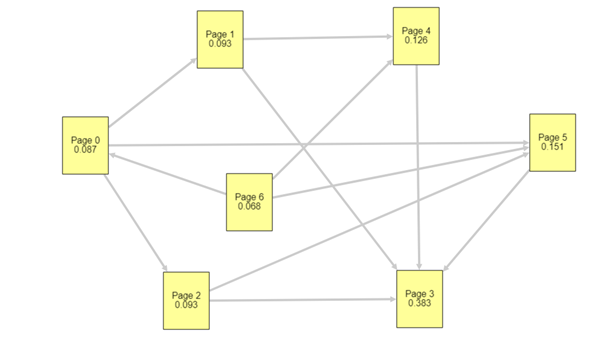
\includegraphics[width=.9\linewidth]{pagegraph.png}
	\caption{A graph representation of webpages and their in and out-links. Algorithms such as Page Rank and HITS use this graph format to help demonstrate their calculations.}
	\label{fig:page}
\end{figure}

For the graph $G = (V, E)$ the webpages can be seen as vertices $v \in V$ with their links as the directed edges between pages, the same way to how they were represented in the HITS formulas. We can let $F_v$ be the set of webpages that $v$ points to, i.e., the forward links. Similarly, the backwards links as $B_v$ which is the set of webpages that points to $v$. The simplified version of Page Rank \cite{page1999pagerank} can then be defined with $N_v = \left|F_v\right|$ in Equation \ref{eq:prb}.

\begin{equation}\label{eq:prb}
PR(v) = c\sum_{w \in B_v}\frac{PR(w)}{N_w}
\end{equation}

where c is a variable used for normalisation purposes so can be modified accordingly. The page rank is calculated by the even distribution of the page rank for webpage $v$ among webpages that $v$ points to. The page ranks that links to other webpages from $v$ are then used to calculate their page rank. Hence giving an iterative approach to calculating their ranks whilst the algorithm travels along the links of the webpages. On the other hand, if a webpage does not have out-links and only in-links from other webpages then their rank is never distributed to others causing its value to accumulate. This situation is known as a \emph{rank sink}.

A remedy to having a rank sink is to use a a damping factor to illustrate the probability that the user follows the links on the webpage. This takes into consideration that users could skip pages or go directly to another webpage that were not linked through the URL. Hence ($1-d$) is considered as the distribution of the page rank from webpages that were not directly linked to it, i.e., no direct edges between them. Thus, for the page $v$ with $b_i \in B_v$, the page rank \cite{brin1998anatomy} is defined through Equation \ref{eq:pr}.

\begin{equation} \label{eq:pr}
PR(v) = (1-d) + d (PR(b_1)/F(b_1) + … + PR(b_n)/F(b_n))
\end{equation}

where $F(v)$ was retrieved from the set $F_v$ for the webpage $v$. Page rank is applied to each page and is repeated on further pages until the equation converges. The damping factor adds randomness into the network of webpages so that the rank sink does not occur and ensures the convergence is not reached too quickly. Usually, the damping factor is taken to be $0.85$. 

By using summation, the Page Rank formula can be simply reduced to

\begin{equation}
PR(v) = (1 - d) + d\sum_{w \in B_v}\frac{PR(w)}{N_w}
\end{equation}

The algorithm for calculating page rank can be modified depending on the use and aims. Such modifications include adjusting the vertex and edge values, modifying the damping factor or introducing a new variable into the algorithm. These such changes are known as \emph{personalisation} and an example of personalisation is the \emph{Weighted Page Rank} \cite{xing2004weighted}. Where larger values are assigned to more popular or important webpages rather than the even distribution that occurred beforehand. Webpages that have out-links will instead receive a value proportional to the page's popularity. Their popularity is based off the number of in-links and out-links they hold. These popularity values of the in-links and out-links are represented by $W^{in}_{v,w}$ and $W^{out}_{v,w}$ respectively. $W^{in}_{v,w}$ is calculated by the in-links of webpage $v$, shown to be $I_v$, and the in-links of all the webpages that the webpage $w$ references. This is represented as a set, and we call this set of pages $R(w)$ with $I_p$ where $p \in R(w)$. Furthermore, with these changes, $W^{in}_{v,w}$ and $W^{out}_{v,w}$ can then be formularised into Equations \ref{eq:prwin} and \ref{eq:prout} respectively.

\begin{equation}\label{eq:prwin}
W^{in}_{v,w} = \frac{I_v}{\sum_{p \in R(w)}}{I_p}
\end{equation}

\begin{equation}\label{eq:prout}
W^{out}_{v,w} = \frac{O_v}{\sum_{p \in R(w)}}{O_p}
\end{equation}

where $O_v$, $O_p$ is defined the same as the in-links previously but with the use of the out-links as a replacement. Therefore, the Page Rank formula can be modified to include the webpage's importance giving us the Equation \ref{eq:proverall}.

\begin{equation}\label{eq:proverall}
PR(v) = (1 - d) + d\sum_{w \in B_v}PR(w)W^{in}_{v,w}W^{out}_{v,w}
\end{equation}

So, this formula is focussed more upon the webpages that are visited more frequently by users and ensures they end up with a higher rank. 

However, for the purpose of general directed weighted graphs, the edge weights are lost in the formula as the algorithm updates the rank of every vertex in each iteration meaning that the weights can be disregarded and replaced with the page ranks instead. To ensure this does not happen, the weights of all the edges must be included in the rank's calculation. This is accomplished by summing up the weight values of the in and out edges and incorporating it into the formula as achieved by Equation \ref{eq:wpr}.

\begin{equation} \label{eq:wpr}
PR(v) = (1-d) + d\sum_{w \in B_v}\frac{PR(w)w_{(w \rightarrow v)}}{N_w}
\end{equation}

where $N_w = \sum_y{A_{w,y}w_{(w \rightarrow y)}}$ is redefined as the sum of weights of the out-linked edges in relation to vertex $w$.
\\

Whilst HITS and Page Ranks are designed for the search engine, the network of webpages essentially is a large directed graph that can contain weights hence why the Page Rank can be used on any derivatives of a weighted directed graph. Thus, these are additional graphical properties that can be used to help analyse the structure and linkage of a graph. 

In conclusion, we take the page rank formulas into the experimentations of linguistic analysis. This is because we do not have the requirements of hubs and authorities as shown in the HITS algorithm, so we use the page ranks for directed graphs in future. In addition to the page ranks, we will incorporate the use of local clustering coefficient, trophic levels and the betweenness centrality so that various graph visualisations can be produced. Before applying these to linguistic data, we begin with initial experimentations on a smaller dataset shown in the next chapter. This is to ensure that the visualisations work and to implement any modifications that may be required. Also gives us further insight as to what various values represent in a different dataset.
